% the one-ring of a vertex cut open and flattened, and rescaled so that it closes up: a cone (300 degrees) and a saddle (420 degrees)
\begin{tikzpicture}[scale=1.15]
  \foreach \k in {0,...,4} {\filldraw[draw=gray!70, fill=gray!12] (0,0) -- ({60*\k}:1) -- ({60*(\k+1)}:1) -- cycle;}
  \draw[red!70!black, dashed] (0,0) -- (0:1.2);
  \fill[red!12] (0,0) -- (300:0.45) arc (300:360:0.45) -- cycle;
  \node[red!60!black, font=\scriptsize] at (330:0.68) {$60^\circ$};
  \node[font=\scriptsize] at (30:0.62) {$60^\circ$};
  \draw[-{Stealth[length=1.8mm]}, thick, blue!70!black] (0,0) -- (0:0.95) node[below right, font=\scriptsize] {$\theta = 0$};
  \fill (0,0) circle (1.2pt);
  \node[below, font=\footnotesize, align=center] at (0,-1.2) {cone, cut open\\$\Theta_i = 300^\circ$};
\end{tikzpicture}\hfill
\begin{tikzpicture}[scale=1.15]
  \foreach \k in {0,...,4} {\filldraw[draw=gray!70, fill=gray!12] (0,0) -- ({72*\k}:1) -- ({72*(\k+1)}:1) -- cycle;}
  \node[font=\scriptsize] at (36:0.62) {$72^\circ$};
  \draw[-{Stealth[length=1.8mm]}, thick, blue!70!black] (0,0) -- (0:0.95);
  \fill (0,0) circle (1.2pt);
  \node[below, font=\footnotesize, align=center] at (0,-1.2) {rescaled by $s_i = \frac{6}{5}$\\closes up};
\end{tikzpicture}\hfill
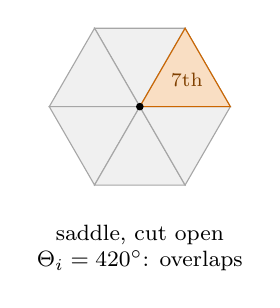
\begin{tikzpicture}[scale=1.15]
  \foreach \k in {0,...,5} {\filldraw[draw=gray!70, fill=gray!12] (0,0) -- ({60*\k}:1) -- ({60*(\k+1)}:1) -- cycle;}
  \filldraw[draw=orange!80!black, fill=orange!35, fill opacity=0.6] (0,0) -- (0:1) -- (60:1) -- cycle;
  \node[orange!50!black, font=\scriptsize, align=center] at (30:0.6) {7th};
  \fill (0,0) circle (1.2pt);
  \node[below, font=\footnotesize, align=center] at (0,-1.2) {saddle, cut open\\$\Theta_i = 420^\circ$: overlaps};
\end{tikzpicture}\hfill
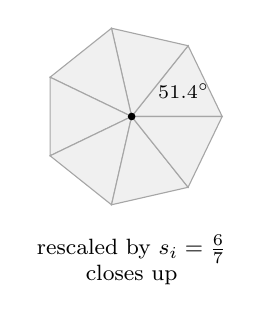
\begin{tikzpicture}[scale=1.15]
  \foreach \k in {0,...,6} {\filldraw[draw=gray!70, fill=gray!12] (0,0) -- ({360/7*\k}:1) -- ({360/7*(\k+1)}:1) -- cycle;}
  \node[font=\scriptsize] at ({180/7}:0.64) {$51.4^\circ$};
  \fill (0,0) circle (1.2pt);
  \node[below, font=\footnotesize, align=center] at (0,-1.2) {rescaled by $s_i = \frac{6}{7}$\\closes up};
\end{tikzpicture}
